\chapter{Introduction}
\label{chap:intro}

\section{Enforcing Security Isolation for Applications}
\label{sec:intro:isolation}

In traditional systems, the security of an application is built upon
trusting the whole system stack to enforce its security policies.
The system stack needed to be trusted
--- as part of the application's {\em trusted computing base (TCB)}
--- includes the hardware (from CPUs to devices), operating systems, system libraries, and language runtimes.
If a vulnerability exists anywhere in the system stack,
attackers can exploit the vulnerability to bypass security mechanisms applied by the application,
compromising any security policies that application applies.

However, as the design of the hardware, operating systems, libraries and runtimes grows increasingly complex,
it becomes harder for system developers to eliminate the vulnerabilities
from the system stacks.
Theoretically, system developers can use debugging or formal verification
to assist or verify the elimination of vulnerabilities.
However, the formal technique cannot be proven perfect, and the latter requires tremendous effort to ensure its correctness
when the whole system stack is huge.

The existence of vulnerabilities in the trusted system stack especially affects applications that run in a multi-tenant environment, such as {\em cloud} environment.
If there is only one tenant,
the application or user will behaves benignly,
without actively attempting to discover or exploit any system vulnerabilities.
On the contrary, in a multi-tenant environment,
the application or user can share the same host with a malicious application or user,
who will act to compromise the system stack.
The problem can never be completely resolved by security checks,
because vulnerabilities can exist in the security logics,
and the attackers who succeed exploiting the vulnerabilities may bypass the checks.

To address the problem of system vulnerabilities, system researchers have engaged efforts in building more secure operating systems,
to isolate the consequence of compromised system stacks.
For instance,
micro-kernels, such as Exokernel~\citep{engler95exokernel} or HiStar~\citep{zeldovich+histar},
intend to reduce the TCB in the operating systems that are shared by applications.
The operating system components that are removed from the shared TCB are placed into a {\em library OS}, which operates in the userspace or even in the application processes.
If a malicious application attack its library OS,
the succeeded exploitation will only affect the very piece of library OS,
whereas other applications are isolated.
Because the complexity of the host kernel is significantly reduced,
it is easier to eliminate its vulnerabilities.

Another common approach of enforcing security isolation against malicious application to use virtualization.
With virtualization, the shared TCB among all the guests (or tenants)
are reduced to a minimal hypervisor,
and each guest will be running in an isolated virtual machine which loads a monolithic guest operating systems.
Similar as the applications isolated by library OSes, the exploitation that occurs in each guest OS will not affect other guests.

Either library OSes or virtual machines does not defend against two types of attacks.
The first type of attack is from the malicious host providers.
In cloud environment, a malicious provider can load a modified kernels or hypervisors into the hosts,
bypassing the security isolation enforced by library OSes or virtual machines.
Even without loading a malicious system stack,
the provider can still attack the hosts by physically launching attacks on the hardware, using techniques such as the Cold-boot Attack~\citep{halderman09coldboot} or 
intrude the boot process using counterfeit peripheral devices.
Finally, library OSes or virtual machines does not defend against vulnerabilities
inside an application or a process
that can be exploited to attack the application itself.
For instance, the Heartbleed bug~\citep{heartbleed} discovered in OpenSSL cryptography library
can leak the private keys of trusted authorities through the vulnerability in OpenSSL's heartbeating service.
To eliminate vulnerabilities in a complex, modern applications is as infeasible as eliminating vulnerabilities in the operating systems.

This thesis primarily describes three security isolation solutions,
to defend against different levels of attack:
\begin{compactitem}
\item {\em \graphene{}} (\S\ref{chap:graphene}) enforces security isolation between mutually untrusting applications.
\item {\em \gsgx{}} (\S\ref{chap:gsgx}) enforces security isolation on applications against untrusted system stacks and other applications.
\item {\em \civet{}} (\S\ref{chap:civet}) enforces security isolation inside an application, against untrusted application partitions as well as the system stacks and other applications.
\end{compactitem}

\section{Security Isolation for Linux Multi-Process Applications\\ using a Library OS}
\label{sec:intro:graphene}

Existing library OSes (\libos{}) enforce security isolation of mutually untrusting process,
at a lower cost than using virtualization
~\citep{porter11drawbridge,unikernels,baumann13bascule}.
More recent \liboses{}
provide several qualitative benefits of virtualization,
such as migration and host platform compatibility.
%Library OSes move portions of
%OS kernel functionality into an application library.
In a \libos{}, the guest OS is essentially ``collapsed''
into an application library, to be loaded into the user memory of application processes ({\em \picoprocs{}}).
%% dp: too early for this nomenclature, I think
% \daniela{(a libraryOS instance)},
A \libos{} implements the OS system calls and supporting data structures as library functions---mapping
high-level APIs onto
a few paravirtual interfaces to the host kernel.
Recent library OSes improve efficiency over full guest OSes by eliminating duplicated features
between the guest and host kernel,
such as the CPU scheduler, or
%eliminating guest-level multiplexing code, as the library OS supports only one application;
even compiling out unnecessary guest kernel APIs~\citep{unikernels}.
In total, this can reduce the memory requirements of running a single, isolated application
by orders of magnitude, and similarly
increase the number of applications which can run
on a single system~\citep{porter11drawbridge,unikernels}.
In addition, \liboses{} have been proven
useful for porting legacy applications
onto new hardware platforms, such as \intel{} \sgx{}~\citep{baumann14haven}.
%% dp: This sentence seems a little premature
%In recent works, library OSes provide rich OS features for isolated contexts while the host OSes are untrusted

%% Library OSes reduce the memory requirements of running a self-contained,
%% isolated application process
%% %guest \daniela{I would replaced guest by "isolated process or group of processes (a libOS instance)''}
%% by orders of magnitude
%% In a cloud computing environment,
%% increasing the number of applications per server has enormous
%% economic benefits.
%% Even on a desktop or portable system, \libos{}es can reduce the overheads
%% of sandboxing untrusted code and running applications
%% designed for another OS.

%Because library OSes execute within a VM \daniela{this phrase does not read good to me because (i) it might imply the picoprocesses need hypervisor support, as misunderstood by reviewer 1 and (ii) you already emphasized the drawbacks of leveraging a VM} or lightweight process ({\em picoprocess}~\citep{xax}),
%library OSes execute with

%% dp: Daniela, great suggestion!  We need to make this situation seem more
%%     like the sky will fall without our help
A key drawback of recent library OSes, however,
is that they are limited to single-process applications.
Yet many applications, such as network servers and
shell scripts,
create multiple processes
for
performance scalability, fault isolation, and programmer convenience.
%These applications would benefit from the efficiency and security benefits
%of a library OS.
In order for the efficiency benefits of \liboses{} to be widely applicable,
especially for unmodified Unix applications,
%either applications must be rewritten to implement ad hoc coordination mechanisms, or
\liboses{} must  provide commonly-used multi-process abstractions,
such as fork,  signals, System V IPC, and exit notification.
To support multi-process abstractions, \liboses{} often have to rely on sharing OS states,
backed by the hosts' memory sharing features.
For example, Drawbridge~\citep{porter11drawbridge} cannot simulate process forking because copy-on-write memory sharing is not a platform-independent features.


%\begin{figure}[t!]
%\centering
%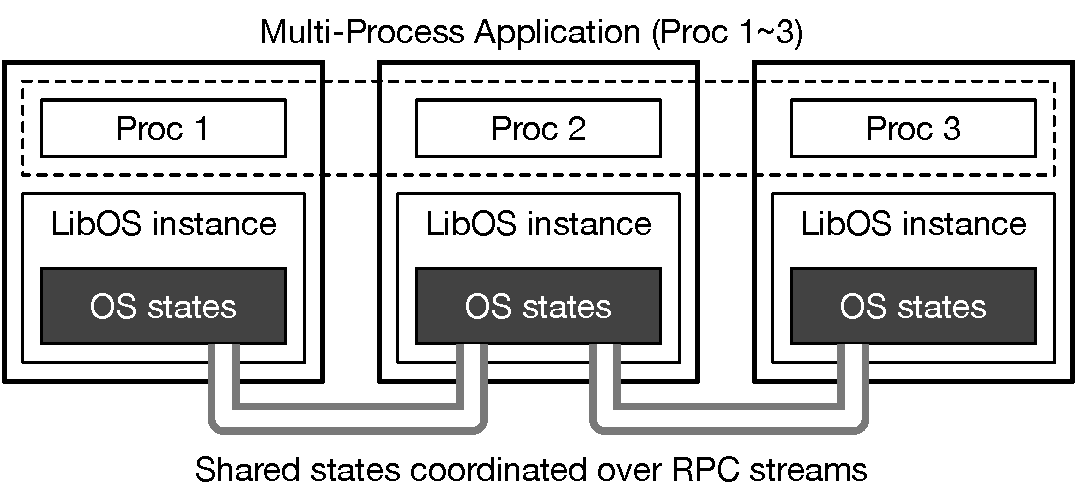
\includegraphics[width=0.75\linewidth]{graphene/figures/concept.pdf}
%\caption[Multi-process abstraction model of \sysname{} \libos{}]
%{Multi-process abstraction model of \sysname{} \libos{}. For each process of an application, a libOS instance will serve system calls and keep local OS states. States of multi-process abstractions are shared by coordinating over host-provided RPC streams, creating an illusion of running in single OS for the application.}
%%\vspace{-.1in}
%\label{fig:graphene:concept}
%\end{figure}

This paper describes {\em \graphene{}}, a Linux-compatible \libos{} to secure unmodified, Linux multi-process applications.
In \graphene{}, multiple \libos{} instances collaboratively implement
multi-process abstractions,
yet appear to the application
as a single, shared OS.
\graphene{} instances coordinate state using remote procedure calls (RPCs) over
host-provided, pipe-like streams.
In a distributed POSIX implementation, placement of shared state and messaging complexity
are first-order performance concerns.
%We chose to shift implementation complexity into the library OS
%in order to uphold simple enforcement of security isolation in the host.
By coordinating shared states across \libos{} \picoprocs{,
\graphene{} is able to create an illusion 
of running in a single OS
for multiple processes in an application.

%Previous library OS designs ensured security isolation of independent applications,
%comparable to a VM, by keeping a relatively narrow host ABI.
%We selected the \sysname{}
%design because it strikes a unique balance between
%and robust, flexible security enforcement.

The design of \graphene{} ensures security isolation of
mutually distrusting, multi-process
applications on the same host.
Essential to this goal is
minimally expanding the host ABI to support multi-processing,
as well as leveraging RPCs as a natural point to mediate inter-\libos{} communication.
RPC coordination among \graphene{} instances can be dynamically disconnected, facilitating novel sandboxing
techniques.  For instance, we develop an Apache web server extension that, upon logging in a given user,
places the worker process's \libos{} in a sandbox with access to only that user's data.
We expect more nuanced degrees of trust are possible in future work.

%\graphene{}'s design gives the user and system administrator a high degree of flexibility
%in isolating arbitrary groups of unmodified application processes,
%while upholding the efficiency and host compatibility benefits of recent \liboses{}.

%\fixmedp{After a complete draft is written, coalesce all goals and make sure they are addressed early on.  We are doing some scatter-shot motivation}

\section{Isolating Native Applications on Untrusted Hosts}
\label{sec:intro:gsgx}

%The complexity of modern operating systems has become
%a major source of security vulnerabilities,
%pressuring developers to seek solutions to exclude the host OSes
%from their trust models.
%The untrustworthiness of OSes get severe when applications are run in the cloud,
%because the applications may cohabit with compromised tenants,
%or be hosted by malicious providers.

Existing works provide isolated execution of applications
on untrusted operating systems or host hardware,
using either hypervisors~\citep{criswell2014virtualghost, flicker, inktag, zhang2012mushi} or security hardware~\citep{intelsgx, secureblue++}.
Especially security hardware such as \intel{} \sgx{}~\citep{intelsgx} can defense against hardware-level attacks,
with low execution overhead.
\sgx{} is a set of new instructions introduced in the latest \intel{} CPUs,
to create a encrypted memory region called {\it enclave}
in the application's address space.
\sgx{} guarantees that only signed code loaded in the enclave can access the sensitive data stored in the enclave memory.

%Protecting applications without the requirement of trusting the hosts
%has become valuable in modern computer systems for many reasons.
%The complexity of the existing monolithic operating systems has become a major source of
%vulnerabilities to exploit.
%Once the host operating systems are compromised,
%any security mechanisms enforced in the applications can be easily circumvented.
%If the applications run in the cloud,
%the hosts have to be controlled by the cloud providers,
%which is capable of compromising both host operating systems and hardwares.
%The attacks from the cloud is possible even if
%the operating systems' vulnerabilities are never exploited.

However, isolating an application with \sgx{} enclaves
requires additional porting effort,
to partition the application into a signed, trusted binary,
and the rest.
Only the trusted binary will be loaded in enclaves.
The enclave will interact with the rest of the application
through an {\em untrusted interface},
to pass input and output of the isolated execution,
and access OS features such as files and network.
For a complex application such as a network server or a desktop GUI,
the effort to partition the application is too high,
and the untrusted interface is often too large,
given the complexity of interaction between the enclave and the rest of the application.

%Unfortunately, leveraging SGX for security
%often requires rewriting the applications to a large extent.
%Because the OSes cannot be trusted,
%enclaves are not allowed to directly access any system interface
%for any OS features
%such as files, networks or scheduling.
%Only a limited subset of system library API can be exported in enclaves;
%for example, the software development kit for SGX
%only supports spin-locking as scheduling tool,
%because other primitives require cooperation from the OS.

With the support of a \libos{}, developers can port an application to \sgx{} with minimal effort,
using a {\em non-partitioned model}~\citep{baumann14haven}.
The non-partitioned model loads the whole application binary into the enclave,
and a \libos{} to support the OS features.
The benefits of using a non-partitioned model also include
limiting the untrusted interface to a narrow, fixed interface,
and the fact that the application is protected ``as is''
--- especially useful for privacy-preserving applications.

%To alleviate the pain of migrating applications to SGX,
%recent works like Haven~\citep{baumann14haven} provides a mechanism
%of loading native applications into enclaves,
%alongside a library OS to facilitate rich OS features.
%These systems are called ``shielding %systems''~\citep{xu15controlledchannel},
%which means these systems can secure execution environments
%without trusting the host.

A primary drawback of the non-partitioned model is the huge TCB loaded into the enclave.
In the partitioned model, only minimal code needed for the isolated execution will be loaded into the enclave.
However, in the non-partitioned model, the whole application must be loaded into the enclave,
in addition to the TCB contributed by the \libos{}.
For instance, size of the \libos{} used in \cite{baumann14haven} is 209MB,
which yields significant expansion to the original TCB.

We present {\em \gsgx{}}, a port of \graphene{} \libos{} on \sgx{}, to secure unmodified Linux applications in \sgx{} enclaves{}.
The support for Linux applications
has been missing in the non-partitioned model,
which is a missed opportunity according to the 75\% market share of Linux cloud providers~\citep{linuxcloud2014}.
\gsgx{} supports most OS features provided by \graphene{}
including both single- and multi-process abstractions.

The design of \gsgx{} ensures the minimal enclave TCB
that can be achieved without further partitioning any application binaries.
The integrity of the loaded application binaries
is enforced in a fine-grained fashion:
each binary must be signed and checked individually,
and only binaries that are actually needed will be ever loaded.
For multi-process applications,
\gsgx{} isolates each \picoproc{} in a separate enclave,
thus every \picoproc{} can execute and be attested separately.
In a nutshell, \gsgx{} tries to honor and exploit the established partitioning in multi-process applications,
with the benefit of minimizing the porting effort from using the non-partitioned model.

\begin{figure}[t!]
\centering
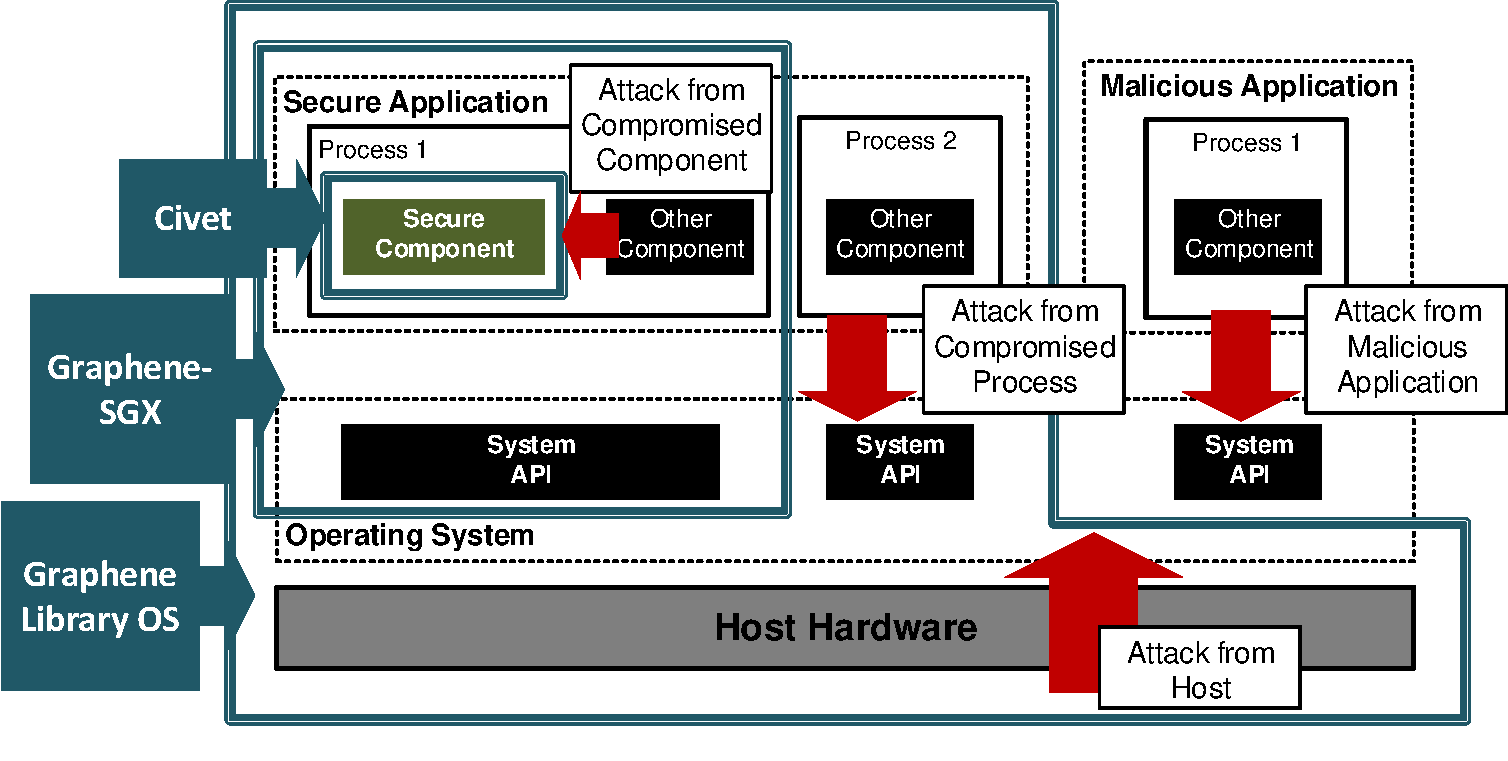
\includegraphics[width=4.5in]{figures/defense.pdf}
\caption[Types of potential attacks on an application, and the TCB required by \graphene{}, \gsgx{} and \civet{}]
{Type of potential attacks on the security of an application and the trusted computing base (TCB) required by \graphene{}, \gsgx{} and \civet{}.
An application can be attacked from either the corrupted host system stack, malicious applications, or compromised components and processes in the application.
\graphene{} can expel all untrusted applications and the system APIs that are affected by them.
\gsgx{} further removes the host kernel and hardware, as well as untrusted processes, from the TCB. \civet{} then defends against compromised, in-process components.}
\label{fig:graphene:arch}
\end{figure}


%
%Haven effectively migrates native Windows applications to enclaves,
%providing a shortcut for developers
%to easily boost the security of their products.
%However, there are several limitations in Haven, including
%excessive trusted computing base (TCB),
%a restrictive model of adapting applications,
%and missing support for Linux or multi-process applications.

%We present \gsgx{}, a \libos{}-based shielding system
%targeting Linux multi-process applications,
%as improvement to the Haven model of migrating native application to SGX.
%\gsgx{} is derived of \graphene{}~\citep{tsai14graphene},
%which supports 139 out of 300 Linux system calls.
%\graphene{} runs numbers of popular applications
%such as Apache web server, OpenJDK virtual machine, or shell scripts,
%all of which relies on multi-process abstractions
%such as {\tt fork}, {\tt execve}, signals or System V IPC.

%By supporting Linux multi-process applications,
%\gsgx{} simply applies to a broader range of cloud-based applications
%than Haven.
%Survey shows that Linux yields a market share of up to 75 percent in
%enterprise cloud providers~\citep{linuxcloud2014}.
%This data suggests majority of the existing cloud users can
%more easily adopt \gsgx{} than Haven.

%\gsgx{} uses a different model from Haven
%to bootstrap the trust of loaded applications.
%Haven builds up the trust by packing all binaries
%in an encrypted virtual disk,
%with secret key provisioned consensually from a remote server
%trusted by the clients.
%Contrastingly, \gsgx{} relies on a model directly derived from
%the trust model of \sgx{},
%by including applications' checksums
%into the enclave measurement to be attested by hardware.
%\gsgx{} can migration applications for enclaves off-line,
%and share binaries (e.g., shared libraries) to save bandwidths for deployment.
%
%Security-wise speaking,
%\gsgx{} provides a way to reduce the TCB of enclaves,
%with a smaller code footprint
%and applications natively partitioned as processes.
%Haven in general yields a large TCB
%including a \libos{} as large as 209MB,
%and application binaries around 10s \textasciitilde 100s of MB.
%The image of \gsgx{} is merely 10MB,
%and Linux applications generally follow the principle of dividing
%code into smaller, more testable binaries.
%\gsgx{} isolates multiple binaries (or processes) of an application
%in separate enclaves, and authenticates inter-process coordination
%by binary-based policies.
%Even if an enclave is compromised, other enclaves of the same application
%can still stay secure as long as
%critical information never flows to the victim.
%
%\gsgx{} provides cloud users
%ease of shielding Linux applications
%and flexibility of implementing any desired security model
%suitable for each binary.

\section{Combining Isolated Execution with Language Protection\\ for Partitioned Applications}
\label{sec:intro:civet}

%% \fixme{Chia-Che Tsai's opening}
%% Modern security hardwares such as TPM or \intel{} SGX
%% provide hardware enforced guarantees of security properties
%% even upon %untrustworthy hosts with
%% compromised operating systems or tampered hardwares.
%% The reasoning of security using these hardwares
%% is often founded as follows:
%% An untamperable hardware package such as CPU will guarantee
%% the integrity of applications loaded
%% exactly identical to the images signed by clients.
%% However, to achieve overall security,
%% the clients are still responsible for ensuring that no vulnerabilities
%% within the signed images
%% will compromise the security properties in runtime.

%\fixmedp{I would start by motivating the goal of application partitioning.
%I think you could add a little more here, but this is a rough sketch.}
For applications that handle sensitive data such as private keys,
or implement proprietary algorithms,
running on a untrusted host whose hardware and hypervisor
may be compromised is a huge risk.
%, such as medical applications, or 
%implement proprietary algorithms, such as algorithmic stock trading.  
%These applications are composed of 
%libraries and other code from third parties, and may run on 
%hardware and hypervisors provided by an untrusted cloud provider.
%Using the partitioned model the developers can 
%bound the effort to protect sensitive data and algorithms,
%while still taking advantage of inexpensive code and cloud hardware.
%A partitioned application isolates sensitive data and code, typically using
%language or hardware techniques.
If users run these applications in isolated execution such as \sgx{},
due to the complexity of the applications,
the cost of partitioning and porting the applications may be too high to pay.
However, as discussed in \S\ref{sec:intro:gsgx},
using the non-partitioned model, the application must tolerate a much larger TCB in the isolated execution,
whereas a large fraction of the TCB is less sensitive.

A solution to this dilemma
is to automate the partitioning using language techniques.
For instance, applications implemented in managed languages like \java{}
are easier to partition,
if a few hints about the sensitive data can be provided by the developers.
Since \java{} classes are often well modularized,
an automated language-level tool can analyze the minimal supporting classes to process the sensitive data,
creating a clean partition with more reasonable TCB.

%%Why SGX
%%\fixme{Bhushan's opening}
%At the hardware level, 
%new CPUs are offering features to protect application-level code and data
%from a  compromised or malicious system software stack,
%including the OS or hypervisor, or simply isolating portions of the 
%application address space from the rest of the application.
%Examples include SX~\citep{sgx-manual}, 
%%\fixmedp{Can we mention/cite others? IBM and ARM?}
%IBM SecureBlue++~\citep{secureblue++}, and ARM TrustZone~\citep{trustzone}.
%%are offering models of mutual distrust, which facilitate protecting
%%an application from a
%SGX offers %One feature of SGX is restricted
%entry points to an encrypted region of memory, called an {\em enclave}.
%Encryption and remote attestation 
%prevent the hypervisor or OS from reading or modifying the enclave's contents,
%and validate that the enclave was correctly initialized.
%This in turn
%can exclude 
%a cloud provider's hypervisor or OS from the application's trusted computing base (TCB),
%requiring only trust in the hardware manufacturer (i.e., Intel).
%%Remote attestation can also validate that an enclave was correctly initialized.
%%Enclaves also provide remote attestation, where a client
%%can ascertain whether the hardware is genuine Intel, and that the application was
%%loaded correctly.
%SGX also offers protection against malicious devices off the CPU package,
%such as a compromised storage device.

Besides automated partitioning,
securing \java{} applications in \sgx{} opens opportunities to hardening the security of isolated execution,
using language-level protections
~\citep{bittau2008wedge,brumley2004privtrans,khatiwala2006data}.
For instance, the type-checking feature in the \java{} language
can avoid the risk of exploitable pointers or control flow errors,
which is significant in an unsafe language like C
~\citep{nergal2001libc,bletsch2011jump,checkoway2010return}.

In addition, although SGX can restrict enclave entry 
to a few predefined entry points,
the developers still have to reason about what the soundness of the
entry-point definitions, protection against malicious inputs,
and the code paths that must not inadvertently leak sensitive data.
For instance, Iago attacks~\citep{iago}, where an OS offers malicious system call return values,
can be notoriously difficult to defend against from an enclave;
although limited countermeasures exist for the OS API (typically with the cooperation of a 
trusted hypervisor)~\citep{kwon2016sego},%\fixmedp{cite the asplos 16 inktag paper},
there are no off-the-shelf defenses against Iago-style attacks from the compromised application code.

%Further, SGX is designed to run a small, native code library inside of a larger
%application; support for running managed languages in an enclave is currently limited.  
%Writing a security-sensitive application in an unsafe
%language like C dramatically increases the risk of exploitable pointer or control flow errors, which ultimately disclose sensitive data or undermine the integrity of the enclave.

%Modern security hardware
%such as  provides hardware protection to applications
%especially the ones deployed in the cloud,
%so that the applications do not have to trust the privileged
%OS layer controlled by the cloud provider. 
%against malicious system stacks, including OS, hypervisors or devices. 
%In principle, these hardware techniques 
%Hardware protection between applications and their hosts is appealing
%in cloud computing, because the cloud client 
%need only trust the 
%the cloud provider's hypervisor can, in principle, 
%be excluded from the application's trusted computing base (TCB).
%These hardware protection is especially essential for cloud computing, due to the multi-tenant environment and potentially compromisable providers.
%\fixme{I want to emphasize it can defend against hardware attack.}
%This type of hardware creates a sanctuary for the most security-sensitive
%components of an application---

%For instance, SGX creates a encrypted memory region 
%called {\em enclave} within the memory space of an application,
%which can only be accessed by verified code from the users.
%\fixme{I rather not emphasize partitioning so early, it's not the only way of using enclave.}
%SGX lets the developer partition the application into two parts --- 
%security sensitive and non-security sensitive parts. The security
%sensitive part of the application is run in an hardware isolated
%sandbox called enclave, while the non-security sensitive part runs
%normally outside the enclave.
%% SGX guarantees not only the integrity of loaded application image,
%% but also the confidentiality
%% of application data, %in enclave,
%% avoiding any information leakage to the untrusted exterior world.
%SGX provides a fail-safe way to prevent information leakage from the enclave:
%by guaranteeing the integrity of a measured %and verified
%application binary
%and the confidentiality of application data in memory.
%the OS or hypervisor are simply stopped from peeking any application data, unless the isolated applications release any information. 

%Language-level techniques can offer more sophisticated insights into how
%to partition the application, as well as stronger protections ~\citep{bittau2008wedge,brumley2004privtrans,khatiwala2006data}.
%%\fixmedp{Can we bless some language-level app partitioning tools here?}
%Similarly, managed languages such as Java, with type-checking,
%can prevent memory corruption attacks,
%while applications developed in C or C++ are often prone to memory-bug exploitation.  
%Because Java is memory safe, it is immune to known control flow attacks, such as return-oriented programming,
%where control flow is manipulated by unsafe writes to return pointers on the stack or function pointers in objects.

%protection prevents applications from being compromised by
%vulnerabilities that exist inside the applications.
%The vulnerabilities include mistakes made by developers, such as semantic and configuration bugs,
%and unbound application behaviors that can be exploited by attackers,
%such as memory attacks or control flow attacks.
%Based on the different languages used by developers,
%applications can be offered stronger language specific security guarantees.

Although combining isolated execution and language protections
is beneficial for partitioned applications,
the synthesization of the two mechanism can be difficult in practice.
%In general, hardware protection and language-level protection 
%provide separate security guarantees.
%Unfortunately, developers often struggle to combine both types of protection, due to the limitations and lack of support for both approaches.
We focus on the combination of \sgx{} and \java{} as a running example:
\sgx{} are designed to run native code that is primarily developed in C or C++.
Without further support, a partitioned \java{} application
cannot be directly loaded into an enclave.
There is also no API support for \sgx{} features in \java{},
making it challenging for \java{} applications to use any \sgx{} features to their advantage.
%Developers often have to create an ad hoc integration of hardware and language-level protection,
%or they are forced to exclusively expose the application between
%attacks from the system stacks and vulnerabilities inside the applications.
The current state-of-the-art of secure more complex applications with \sgx{} is to develop ad hoc solutions that target specific use cases.
% approaches of combining
%language and hardware protection often rely on ad-hoc solutions that
%are specific to certain use cases or technologies.
For example, \cite{vc3} use \sgx{} to secure data analysis in a MapReduce framework supporting C++
--- instead of the Hadoop framework that generally supports \java{}.

%% dp: this sentence seems off track, unless you want to say something about ``this has to be in C''
%Similarly, S-NFV uses SGX to isolate states of Network Function Virtualization Applications~\citep{shih2016s}.

%\fixmedp{Please check the previous 2 sentences for accuracy; if I'm wrong, try to say something more crisp.
%Also, any other important related work here?}
%to utilize SGX hardware in language runtimes,
%a set of APIs may be exported through the native interface to support certain high-demand use cases, such as Hadoop workloads
%Although these existing solutions nicely support a part of the users,
%and potentially have demonstrated some common wisdom for combining the language and hardware protection,
%the problem of how to generalize the approach
%to cover more use cases or technologies that the authors haven't forseen,
%still remains unsolved.

%% dp: This paragraph is a little too much philosophy for me.  Cutting for now, but can bring some fo this back later in the intro if needed.  I think it would be better for explaining the benfits of Civet.
\begin{comment}
We use SGX vs Java-based protection as an example,
to show how the guarantees ({\em what is secured?})
and features ({\em how is it secured?}) of hardware protection
can be properly modeled at the language level,
so that language protection mechanisms can be extended
to mitigate vulnerabilities in hardware protection. 
For instance,
SGX hardware provides isolation between multiple
levels of security sensitivity in an application process,
by building another privilege level that bypasses the OS or hypervisor.
We model this hardware guarantee at language level by asking the developers
to identify the multi-level security sensitivity in the application.
The developers do not have to worry about
when to enter or leave the enclaves,
what information to flow out of the enclaves,
or even how SGX enclaves fundamentally work.
The language features
such as implicit and explicit information flow tracking can be {\em leveraged}
by the low-level component that interfaces with SGX enclaves
as the criterion for whether certain information
is safe to be released from the enclave.
\end{comment}
%while 
%


%to the privileged
%or un-privileged code outside the \enclave{}.

%One of the primary concerns on the security of enclaves is
%the strong assumption
%that enclaves' security guarantees rely on---
%The security guarantees of hardwares like SGX rely on a strong assumption:
%To provide the confidentiality guarantees,
%the code running in an enclave must not
%the secured environment (\enclave{}) must not
%have %any bugs or
%vulnerabilities that can be exploited for causing any information leakage.
%However, without language support, it is hard to ensure that
%the enclave code is
%free of vulnerabilities, especially if written in C---which provide no memory safety.
%the SGX only supports programs 
%written in C or C++, and it is extremely difficult to find
%all the memory corruption bugs in the enclave code written in C or C++.
%Without memory safety, 
%the control flow of the code %within the enclave
%can be manipulated by exploiting memory corruption.
%This type of vulnerabilities will lead to information leakage,
%defeating the purpose of using SGX enclaves.
%secure hardware such as
%SGX in the first place. 


%% Lack of memory safety using C or C++ in SGX-secured environments \fixme{maybe spell out why it's hard for SGX}
%% enervates any software approaches to reinforce application security, including control flow and information flow integrity, 
%% %These memory corruption bugs can be exploited to change the control flow within the \enclave{} 
%% %as well as leak confidential information outside the \enclave{},
%% defeating the purpose of using %SGX
%% secure hardware in the first place. 
%% \fixme{perhaps justify why not use verification?}

%One solution to guarantee memory safety in applications is to use 
%Using a managed language such as Java
%to implement the security sensitive code
%is a solution to guarantee
%can provide the memory safety
%required by an enclave.
%The solution to avoid the memory corruption bugs is to use a memory safe managed
%language like Java. Thus, partitioning an application written in language such as 
%Java and running the Java based security-sensitive code in an \enclave{}
%can help provide the control flow as well as information flow guarantees that SGX is
%designed for.
%Moreover, Java is widely used to develop many enterprise applications,
%that can improve their security guarantees by leveraging the SGX feature.
%However,
%in absence of Java language support for SGX enclave, 
%it is cumbersome to leverage security guarantees of SGX directly,
%unless developers 
%rewrite the security-sensitive components in C or C++, 
%and integrate %this new code with the original application using a 
%using a foreign function interface such as Java Native Interface (JNI).
%Java Native Interface (JNI).
%to integrate with the rest of the enterprise application.
%Moreover,
%Reimplementing the security-sensitive components
%of the application 
%in C or C++
%Rewriting in C or C++ 
%essentially voids any security benefits brought by managed languages.
%the memory safety guarantees provided by Java. 

%Additionally, having runtime support for SGX in %a managed language like
%Java
%has many benefits.
%Code written in Java %a managed language
%is easier to 
%modularize, partition and reason about the security and information flow.
%Thus, providing Java runtime support for SGX can help provide stronger security guarantees
%for applications running in an \enclave{} as well as make numerous applications
%written in Java secure against shared vulnerabilities of the privileged layer.
%Also, imported library classes can be also secured when used in applications instead of be blindly trusted.
%\fixmebj{Find one more benefit of using Java.} 
%Moreover,
%Java is widely used to develop many enterprise applications,
%which can benefit from the security guarantees of SGX
%without the cost of reimplementation.
%that can improve their security guarantees by leveraging the SGX feature.

%Another notable impediment for effectively leveraging SGX 
%feature in a managed language
%is the trouble developers
%have to endure to partition an existing application into two clear parts and design the interface
%between these two parts. There is a very good chance that an unsuspecting developer may copy
%information which is either security sensitive or derived from security sensitive data to outside 
%the enclave,
%undermining the hardware security guarantees provided by SGX. Thus, we need an 
%easy to use language runtime support for SGX
%that can shield the developer from the complexity of determining whether security sensitive information 
%is leaked outside the enclave.

We present {\em \civet{}}, a framework that combines the benefits of
\sgx{}'s isolated execution and the language protection from \java{}, to protect partitioned applications.
The design of \civet{} avoids the downsides of taking either approach in isolation.
\civet{} includes three primary parts:
a tool that automates the partitioning of applications, ultimately generating an enclave image that includes
the minimal supporting classes;
a runtime framework that verifies and loads the supporting classes into an enclave, and enforces information flow control on the enclave border;
and \java{} APIs to seamless access the \sgx{} features such
as attestation and secure provisioning.
The building block the the \civet{} framework uses \gsgx{} to run a reduced \java{} VM, to load the framework and the trusted classes.
%\fixme{Bhushan, read until here.}
%a framework that help Java developers partition their code
%between security sensitive and non-security sensitive parts by adding a few lines of annotations.
%The framework automatically partitions the code into two separate binaries which are run 
%inside and outside the enclave such that the least amount of code as indicated by the
%developer annotations is run inside the enclave, and transparently creates 
%the necessary interface between the two parts. 
%% The interaction between the 2 parts of the application
%% is handled using \emph{reflection library}.
%% We perform dynamic information flow tracking 
%% and control the information flow at the endpoints of the \enclave{}.
%% By default, the framework automatically encrypts any object leaving the \enclave{}, but the
%% developer can override an endorser method to explicitly let some objects pass in the clear --- e.g.,
%% a ciphertext object. Based on information flow tracking, if an endorsed object is affected by some other
%% security sensitive data before leaving the enclave, the developer has to endorse it again.
%We use dynamic information flow tracking to enforce the policy that no information that is security sensitive or
%derived from other security sensitive information is flowing out of enclave in clear, without explicit
%developer directive.
%% Our framework provides ease of partition as well as makes it explicitly clear to the
%% developer when some information is flowing out of enclave in clear. 
%This ease of use and explicitness helps
%developer reason about the security of the code more clearly.
%Civet achieves three properties: {\em security}, {\em practicality} and {\em usability}.
%Civet is designed to protect the confidentiality and integrity of 
%real-world application code. 
%Civet not only requires very little developer effort to adopt, but also provides the developer
%with essential insights into how data can flow through the application,
%leading to better reasoning about the isolation properties of the partition.
%low developer effort,
%requires minimal porting effort,
%and provides ease of reasoning about the security strength.

%\fixmedp{I would refocus a bit on the contributions.  Make sure I don't overstate}
%Civet addresses design challenges at both the hardware and language level.
%%one from each of hardware protection and language-level protection.
%To extend hardware protection, Civet contributes techniques for dynamically loading JAVA classes in enclaves
%with the same code integrity verification as native, static binaries.
%Civet uses the \graphene{} library OS~\citep{tsai14graphene} to facilitate 
%running a restricted JVM runtime in an enclave.
%to facilitate and restrict the interface size of a 
%and prove the measurement of loaded classes as part of the hardware-generated attestation.
%Then Civet verifies and attests loaded JAVA classes on the basis of measurement checking and attestation generation from the hardware.
%On the other hand, Civet has to adopt language-level protection to enforce information flow policies against leakage over the border of enclave.
%Civet enforces information flow policies at the border of the enclave by incorporating
%Phosphor~\citep{bell2014phosphor} instrumentation on all classes in the enclave,
%tracing both explicit and implicit flows from any confidential data,
%and preventing tainted information from leaving the enclave by any interface, 
%except via explicit declassification by the developer.
%either through exported API or low-level interfaces.

%We implemented the prototype for this framework and show three case studies 
%where this framework can improve security of existing Java applications. 
%Firstly, we show how to isolate a security sensitive library like 
%Bouncycastle in the enclave, so that it does not leak the secret key 
%used for cryptography irrespective of any bugs in the other part of the code.
%Secondly, we use this framework to achieve code confidentiality
%for any closed source library implementing proprietary or secret algorithm.
%Finally, we use the enclave to protect security critical data of a Java Web Start (JavaWS) application.

%As a proof-of-the-concept, 
We study three classic use cases of \civet{}.
The first use case is to isolate the 
session keys and supporting cryptography library in an SSH client and server.
%in which the  used for encrypting the connection
%is partitioned and isolated from the rest of the application, %in the enclave,
%protecting the generated session key while still
%using it for encryption and decryption.
The second use case is a Hadoop workload that run a proprietary algorithm;
the components of the workload (e.g., mapper and reducer)
are securely provisioned from a trusted server.
%Partitioner%\fixmedp{what is this?},
%Mapper, Combiner and Reducer classes are provisioned from a trusted server, protecting confidentiality of the sensitive code.
%always runs in an enclave.
%protecting the confidentiality of the running algorithm.
The third use case is a data manager developed as a web application, which can be deployed through a website.
%---a building block for medical and other applications that handle sensitive data; 
%we protect the secret client data in an enclave on the client's machine.
%\fixmedp{can we explain a bit more about the security property of interest?}
%which can serve as a web application for a website.
For each use case, we show that developers can utilize \civet{} to partition the applications with minimal effort,
and only basic understanding of the isolated execution,
not the cumbersome hardware details.  %n{high-level understanding  knowledge of %almost no familiarity with how 
%the SGX hardware.

%Civet prevents any bugs either in the untrusted application or the isolated crypto library to cause leakage of the encryption key.
%Another use case is a Hadoop job that is provisioned with a secret algorithm, and automatically encrypts computation results
%to eliminate risks of leaking the secret sauce.  

\section{Exploring Practicality}

Besides designing practical solution of security isolation,
we obtain several insights about balancing other system properties
that are critical to the applications.
At the center of the problem is the compatibility requirement by the applications.
We observe that operating system development is bound by compatibility requirements such as implementing the specifications or the API support, and the requirement can impact the development of other system properties.

For instance, during the development of \graphene{}, we observe that the lookup hit latency of file system directory cache is suboptimal,
due to the requirement of checking directory permissions.
We redesign the logic of
directory cache lookup, in both Linux and \graphene{},
to significantly improve the hit latency without breaking any compatibility requirements.
As another example, we observe that the measurement of bug-for-bug compatibility in operating systems causes difficulty in improving the APIs for better security or portability,
as well as evaluating the completeness of a system prototype.
We create more reasonable measurements
that reflect the impact or progress of API implementation,
and use the measurements to evaluate and improve the API support in \graphene{}.
The former study is described in \S\ref{chap:dcache}, and the latter study is in \S\ref{chap:syspop}.


\section{Derived Principles and Future Works}